\documentclass[a4paper]{article} 
\usepackage{graphicx} 
\usepackage[ngerman]{babel} 
\usepackage[ansinew]{inputenc} 
\usepackage[T1]{fontenc} 
\usepackage{tgpagella} 
\usepackage{geometry} 
\usepackage{color} 
\usepackage{microtype} 
\usepackage{minted}
\usepackage{caption}
\usepackage[headsepline,footsepline]{scrpage2}
\usepackage{textcomp}
\usepackage{pdfpages}
\usepackage{mdframed}



\makeatletter
\renewcommand\minted@pygmentize[2][\jobname.pyg]{
  \def\minted@cmd{pygmentize -l #2 -f latex -F tokenmerge
    \minted@opt{gobble} \minted@opt{texcl} \minted@opt{mathescape}
    \minted@opt{startinline} \minted@opt{funcnamehighlighting}
    \minted@opt{linenos} -P "verboptions=\minted@opt{extra}"
    -O encoding=UTF-8,outencoding=iso-8859-1 -o \jobname.out.pyg #1}
  \immediate\write18{\minted@cmd}
  % For debugging, uncomment:
  %\immediate\typeout{\minted@cmd}
  \ifthenelse{\equal{\minted@opt@bgcolor}{}}
   {}
   {\begin{minted@colorbg}{\minted@opt@bgcolor}}
  \input{\jobname.out.pyg}
  \ifthenelse{\equal{\minted@opt@bgcolor}{}}
   {}
   {\end{minted@colorbg}}
  \DeleteFile{\jobname.out.pyg}}
\makeatother


\title{Dokumentation - 6 Übung}
\author{Roman Lumetsberger}
\date{\today}

\newmintedfile[ccode]{cpp}{
               linenos,
               numbersep=5pt,
               frame=lines,
               framesep=2mm
}

\newmintedfile[javacode]{java}{
               linenos,
               numbersep=5pt,
               frame=lines,
               tabsize=2,
               framesep=2mm,
}
\newmintedfile[csscode]{css}{
               linenos,
               numbersep=5pt,
               frame=lines,
               tabsize=2,
               framesep=2mm,
}
\newmintedfile[sqlcode]{sql}{
               linenos,
               numbersep=5pt,
               frame=lines,
               tabsize=2,
               framesep=2mm,
}
\captionsetup{
  font=footnotesize,
  justification=raggedright,
  singlelinecheck=false
}


\newcommand{\srcDir}{../Beispiel/src/at/lumetsnet/caas/}
\newcommand{\testDir}{../Beispiel/test/at/lumetsnet/caas/test/}

\definecolor{lineColor}{RGB}{151,0,0}
\pagestyle{scrheadings}
\clearscrheadfoot
\begin{document}
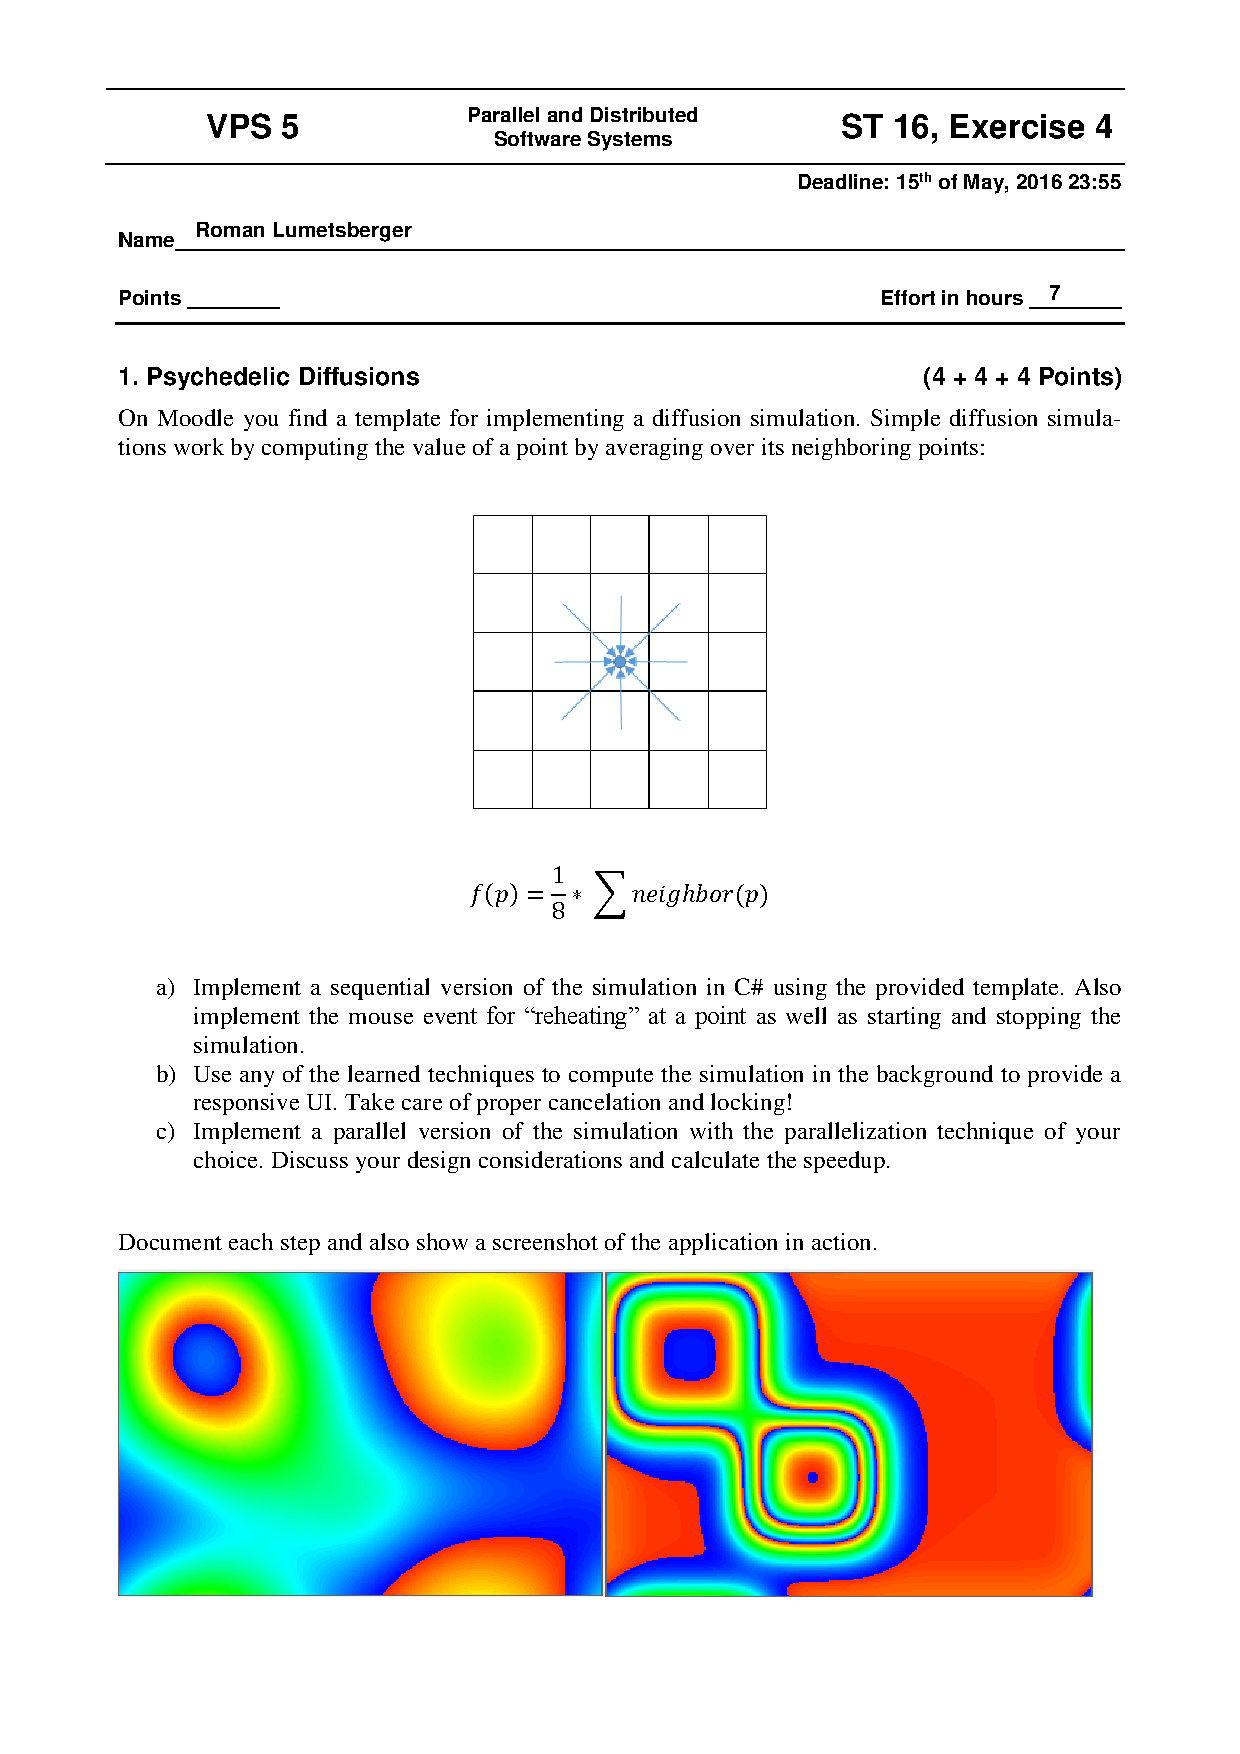
\includepdf[pages=-]{angabe.pdf}

\ihead{VPS SS 2016 - �bung 04}
\ifoot{Roman Lumetsberger}
\cfoot{1310307026}
\ofoot{Seite \pagemark}

\section{Psychedelic Diffusions}
\subsection*{1a. Sequenzielle Version}
Diese Aufgabe wurde bereits in der �bung programmiert und um das Stoppen und Reheating erweitert. F�r die Implementierung selbst wurde eine Basisklasse \texttt{ImageGenerator} erstellt, die die Zeitmessung
und das Ausl�sen des Events �bernimmt. Weiters wurde das Abbrechen �ber ein Stop-Flag \texttt{StopRequested} implementiert. Das Reheating wird mit Hilfe einer \texttt{BlockingQueue} erm�glicht. Diese 
Queue sammelt alle Reheating-Aufrufe w�hrend einer Iteration und wendet sie dann vor Begin der n�chsten Iteration auf die aktuelle Matrix an. 

Der \texttt{SyncImageGenerator} implementiert dann nur noch die Logik zur Erzeugung der n�chsten Matrix und Berechnung der Farben.

\cscode{\srcDir/DiffusionsForStudents/Diffusions/ImageGenerator.cs}
\cscode{\srcDir/DiffusionsForStudents/Diffusions/SyncImageGenerator.cs}

\subsection*{1b. Berechnung im Hintergrund}
Um die Berechnung in den Hintergrund zu verlagern, wurden die Statements in der Methode \texttt{GenerateImage} in einen Task gekapselt und dann mit \texttt{await} auf die Beendigung gewartet. Dadurch wird
der UI-Thread nicht blockiert und die GUI bleibt bedienbar. Auf Synchronisierungsprobleme und die M�glichkeit zum Abbrechen wurde bereits bei der Implementierung 1a R�cksicht genommen.

\textbf{Sourcecode siehe 1.a}

\subsection*{1c. Parallele Version}
Da die Berechnungen der einzelnen Felder der neuen Matrix vollkommen unabh�ngig voneinander sind, ist es m�glich die Schleifen paralell ablaufen zu lassen. Dabei m�ssen keine Synchronisierungen durchgef�hrt werden.
F�r die Implementierung eignet sich die TPL besonders gut, da hier eine parallele Version der For-Schleife angeboten wird. Da der paralell ausgef�hrte Code nicht umfangreich ist, wird zus�tzlich ein \texttt{Partitioner} eingesetzt, da sonst der Overhead zu gro� und eventuell die paralelle Version langsamer als die sequenzielle Version sein w�rde.

Die Klasse \texttt{ParallelImageGenerator} ist wieder von \texttt{ImageGenerator} abgeleitet und implementiert die Berechnung der neuen Matrix mit Hilfe der TPL. 

\cscode{\srcDir/DiffusionsForStudents/Diffusions/ParallelImageGenerator.cs}

\subsubsection*{Performance}
\textbf{Parameter}
\begin{itemize}
\item DisplayInterval: 10
\item MaxIterations: 200
\item Size: 335x224
\item kein Reheating
\end{itemize}

\begin{table}[!htb]
\centering
\caption{Ergebnisse}
\begin{tabular}{ccc}
\hline
\multicolumn{3}{c}{Simulation} \\ \cline{1-3}                                                                                 
Lauf & Sync [ms] & Parallel [ms] \\ \cline{1-3}
1 & 8566 & 7870 \\
2 & 8398 & 8060 \\
3 & 8474 & 7970 \\
4 & 8469 & 7900 \\
5 & 8451 & 8056 \\
\textbf{�}    & \textbf{8471} & \textbf{7971} \\
Std. Abw.    & 54,34      & 77,95

\end{tabular}
\end{table} 

\begin{itemize}
\item SpeedUp: 1,06277
\end{itemize}
Beim Speedup von 1,06277 zeigt, dass Paralellisierung hier nicht viel bringt, da die Berechnung der neuen Matrix nicht wirklich aufwendig ist.

\pagebreak
\subsubsection*{Screenshots}
\begin{figure}[!htb]
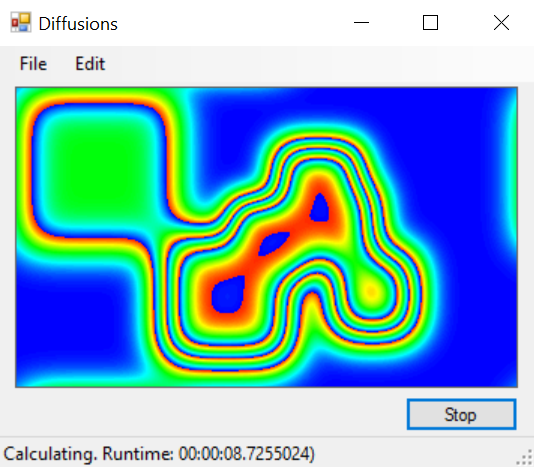
\includegraphics[width=150px]{images/1c_1.png}
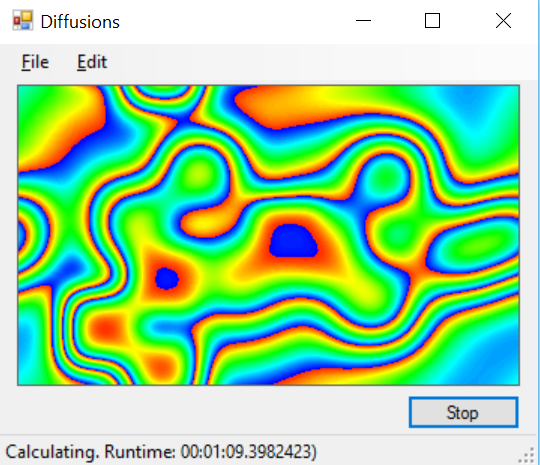
\includegraphics[width=150px]{images/1c_2.png}
\caption{Screenshots}
\end{figure}


\section{Stock Data Visualization}
\subsection*{2a. Asynchrone Version}
Die asynchrone Implementierung verwendet die TPL, um die gew�nschte, paralelle Abfolge zu erreichen. Dazu wurden die synchronen Methoden um asynchrone Versionen erg�nzt. Diese liefern anstatt des
Ergebnisses einen Task zur�ck, auf den dann gewartet und mit \texttt{ContinueWith} weitergearbeitet werden kann. Die asynchrone Implementierung wurde in der Methode \texttt{ParallelImplementation} umgesetzt.

Zuerst wird ein Management-Task gestartet, um das GUI nicht zu blockieren. Dieser Task erstellt dann drei weitere Tasks, die paralell die B�rsedaten abrufen. F�r jeden dieser Tasks werden dann zwei
weitere Task gestartet, die paralell die Kurve bzw. den Trend berechnen. Der Management-Task wartet dann auf alle Ergebnisse und zeigt diese dann im GUI an. Dazu wurde dem Task der \texttt{Scheduler}
des UI-Threads mitgegeben, um die Continuation am UI-Thread auszuf�hren und somit die GUI-Controls updaten zu k�nnen.

\pagebreak
\textbf{Async Versionen der Methoden}
\begin{minted}[
frame=lines,
fontsize=\footnotesize,
tabsize=2
]{csharp}
private Task<StockData> RetrieveStockDataAsync(string name)
{
		return Task.Factory.StartNew(() => RetrieveStockData(name));
}
private Task<Series> GetSeriesAsync(List<StockValue> stockValues, string name)
{
		return Task.Factory.StartNew(() => GetSeries(stockValues, name));
}
private Task<Series> GetTrendAsync(List<StockValue> stockValues, string name)
{
		return Task.Factory.StartNew(() => GetTrend(stockValues, name));
}
\end{minted}

\textbf{Paralelle Version}
\begin{minted}[
frame=lines,
fontsize=\footnotesize,
tabsize=2
]{csharp}
private void ParallelImplementation()
{
		displayButton.Enabled = false;
		Task.Factory.StartNew(() =>
		{
				var seriesList = new List<Series>();
				var tasks = new List<Task>();
				foreach (var name in names)
				{
						tasks.Add(RetrieveStockDataAsync(name).ContinueWith(x =>
						{
								var seriesTasks = new Task<Series>[2];
								seriesTasks[0] = GetSeriesAsync(x.Result.GetValues(), x.Result.name);
								seriesTasks[1] = GetTrendAsync(x.Result.GetValues(), x.Result.name);
								Task.WaitAll(seriesTasks);
								seriesList.Add(seriesTasks[0].Result);
								seriesList.Add(seriesTasks[1].Result);
						}));
				}
				Task.WaitAll(tasks.ToArray());
				return seriesList;
		}).ContinueWith(x =>
		{
				DisplayData(x.Result);
				SaveImage("chart");
				displayButton.Enabled = true;
		}, TaskScheduler.FromCurrentSynchronizationContext());
}

\end{minted}

\subsection*{2b. Asynchrone Version mit async/await} 
Die \texttt{async/await} Implementierung verwendet wieder die Async-Versionen der Methoden, da diese einen \texttt{Task} zur�ckliefern, auf den mit Hilfe von \texttt{await} gewartet werden kann. 
Die Implementierung ist �hnlich der von 2a, doch anstatt von ContinueWith wird await verwendet. Dazu wird wieder f�r jede Aktie ein Task erstellt und in eine Liste gespeichert. Jeder dieser Tasks holt 
sich dann die B�rsendaten durch den Aufruf von \texttt{RetrieveStockDataAsync}. Mit Hilfe von await wird auf das Ergebnis gewartet. Danach folgen die paralellen Aufrufe von \texttt{GetSeriesAsync} und \texttt{GetTrendAsync}.
Diese werden dann durch den Aufruf von \texttt{await} wieder synchronisiert. 

Der Aufruf \texttt{await Task.WhenAll} wartet schlie�lich auf den Abschluss aller Haupttasks und danach kann das Ergebnis in der GUI angezeigt werden.

\pagebreak
\textbf{Async/Await Implementierung}
\begin{minted}[
frame=lines,
fontsize=\footnotesize,
tabsize=2
]{csharp}
private async void ParallelAsyncAwaitImplementation()
{
		var seriesList = new List<Series>();
		displayButton.Enabled = false;

		var tasks = names.Select(GetDataAsync).ToList();
		await Task.WhenAll(tasks);
		tasks.ForEach(x => seriesList.AddRange(x.Result));
		DisplayData(seriesList);
		SaveImage("chart");
		displayButton.Enabled = true;
}

private async Task<List<Series>> GetDataAsync(string name)
{
		var seriesList = new List<Series>();
		StockData data = await RetrieveStockDataAsync(name);
		Task<Series> seriesTask = GetSeriesAsync(data.GetValues(),
				data.name);
		Task<Series> trendTask = GetTrendAsync(data.GetValues(),
				data.name);

		seriesList.Add(await seriesTask);
		seriesList.Add(await trendTask);
		return seriesList;
}
\end{minted}

\end{document}